\chapter{Validierung}
Die in \autoref{Umsetzung} beschriebene, erfolgreiche Umsetzung des in \autoref{Konzept} erstellten Konzepts anhand der in \autoref{Anwendungsszenarien} beschriebenen Szenarien bestätigt die Bedrohungen (\autoref{Analyse:Bedrohungen}), welche auf Industrie 4.0 Netze und deren genutzte Protokolle wirken. Die in \autoref{Analyse} durchgeführte Analyse des in Industrie 4.0 Umgebungen genutzten Netzwerkstacks anhand des \ac{TCP}/\ac{IP} Referenzmodell lieferte Erkenntnisse über mögliche Angriffsvektoren bestehender Systeme, welche durch Inkompatibilität oder Ressourcenmangel ergründet werden können sowie beim Einsatz neuer Technologien und Protokolle des \ac{IIoT}, wenn diese nicht ausreichend für die benötigte Sicherheit der Datenübertragung konfiguriert sind, auftreten. Die Abhängigkeit der Industrie 4.0 Netzwerke auf der \ac{IP} Netzwerktechnologie sorgt für eine Verschmelzung von Produktions-, Office- und Heimnetzen und deren Komponenten. Zur Bereitstellung der \ac{IP} Netze in der Industrie werden somit auch die Dienste des \ac{IP} Protokolls genutzt. Diese Dienste besitzen bekannte Schwachstellen, welche ausgenutzt werden können, um die Kommunikation im Netzwerk zu manipulieren und die Sicherheit zu beeinträchtigen. 

Da eine Beibehaltung der Containerarchitektur des Systems wie in \autoref{arg} beschrieben aufgrund von Softwarebeschränkungen nicht möglich war, wurde das System, um das gewünschte Ziel zu erreichen um weitere \ac{VM}s erweitert. Um vollständigen Zugriff auf die von \ac{IP} genutzten Dienste wie \ac{DHCP} und \ac{DNS} und die Netzwerkadapter der vorhandenen Komponenten zu erhalten und das System so nah als möglich an einer realen Umgebung zu orientieren, wurde die Netzwerkkommunikation des Testsystems von der Containervirtualisierung auf virtuelle Netzwerke der \ac{VM}s verlagert. Dem bestehenden System wurden zwei neue \ac{VM}s hinzugefügt. Eine \ac{VM}, welche die Dienste \ac{DHCP} und \ac{DNS} im Netzwerk übernimmt und das Routing zwischen verschiedenen Netzen bereitstellt sowie eine weitere Komponente, welche als Darstellung eines Systems in einem getrennten Netzwerk dient.

Das Testsystem konnte nach Änderung der Netzwerkarchitektur und Einführung neuer \ac{VM}s um die in \autoref{Anwendungsszenarien} beschriebenen Anwendungsszenarien erfolgreich erweitert werden und somit das in \autoref{Konzept} erstellte Konzept validiert werden. Die Ergebnisse der Anwendungsszenarien können anhand der übertragenen Pakete mit Hilfe des Paketanalysetools Wireshark\footnote{Wireshark - https://www.wireshark.org/} untersucht sowie durch das \ac{GUI} des \ac{CoAP} Monitoringsystems visualisiert werden. Da die gewählten Anwendungsszenarien in keinem direkten Bezug zueinander stehen und keine gegenseitigen Abhängigkeiten besitzen, werden im folgenden die Ergebnisse der Umsetzung einzeln beschrieben.

Das in \autoref{Anwendungsszenarien:OPC UA Kommunikation} beschriebene Anwendungsszenario beinhaltet die Erweiterung der im Testsystem vorhandenen Implementierung des \ac{OPC UA} Protokolls. Nach der Erweiterung des Quellcodes um die Konfigurationsmöglichkeit der \textit{Security Policy}, ist es möglich die Kommunikation zwischen den \ac{OPC UA} Komponenten verschlüsselt und unverschlüsselt durchzuführen. Der Netzwerkverkehr der Docker Container des Testsystems wird über eine Software Bridge durchgeführt. Durch die Paketanalyse des Verkehrs an dieser Stelle ist es möglich die Kommunikation der Komponenten miteinander zu untersuchen. 

Die Abbildungen \autoref{Analyse:opcua-secure-none-req} und \autoref{Analyse:opcua-secure-none-res} zeigen die Ergebnisse der Paketanalyse mit der \textit{Security Policies} "`none"'. Der \ac{OPC UA} Client des Containers "`control"', welcher die Liste der im Netzwerk vorhandenen \ac{OPC UA} Server abfrägt besitzt die \ac{IP}-Adresse 172.18.0.6, der Container des \textit{Discoveryservers} die \ac{IP}-Adresse 172.18.0.2. In \autoref{Analyse:opcua-secure-none-req} ist der Request des Containers "`control"' zum Aufbau eines \textit{Secure Channel} dargestellt. Die verwendete \textit{Security Policy} ist im Bereich "`SecurityPolicyUri"' des \ac{OPC UA} Protokolls beschrieben. In \autoref{Analyse:opcua-secure-none-res} ist die Antwort des \ac{OPC UA} Discovery Servers im \textit{Secure Channel} dargestellt. Es ist zu erkennen, dass die Kommunikation, obwohl der \textit{Secure Channel} genutzt wird, nicht verschlüsselt ist. Die Endpunkte sowie deren Adressen und bereitgestellte Methoden können aus den Paketen ausgelesen werden.

In den Darstellungen \autoref{Analyse:opcua-secure-sha-req} und \autoref{Analyse:opcua-secure-sha-res} wird erneut das Abfragen des Containers "`control"' aller im Netzwerk vorhandenen Endpunkte beim \ac{OPC UA} \textit{Discoveryserver} mit Hilfe eines Request und der dazugehörigen Response beschrieben, jedoch wird das Sicherheitsprofil "`Basic256Sha256"' mit dem \textit{MessageSecurityMode} "`SIGNANDENCRYPT"' genutzt. Der \ac{OPC UA} Client besitzt die \ac{IP}-Adresse 172.18.0.7. Der \textit{Discoveryserver} weiterhin die Adresse 172.18.0.2. Es ist zu erkennen, dass der gesamte Netzwerkverkehr im \textit{Secure Channel} durch den Algorithmus SHA256 verschlüsselt wurde.

\begin{figure}[h]
  \centering
  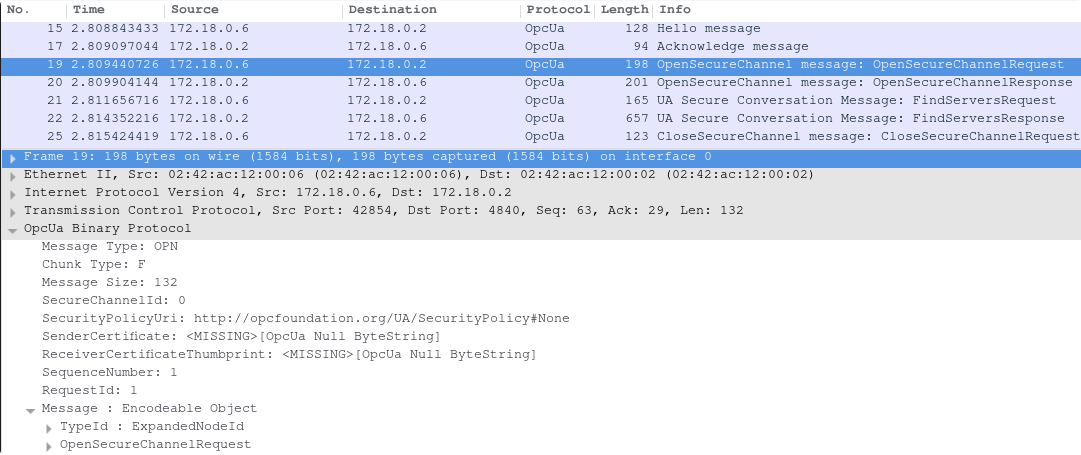
\includegraphics[width=14cm]{opcua-secure-none-req}
  \caption{Paketanalyse OPC UA - Client Request bei Sicherheitsprofil "none"} 
  \label{Analyse:opcua-secure-none-req}
\end{figure}

\begin{figure}[h]
  \centering
  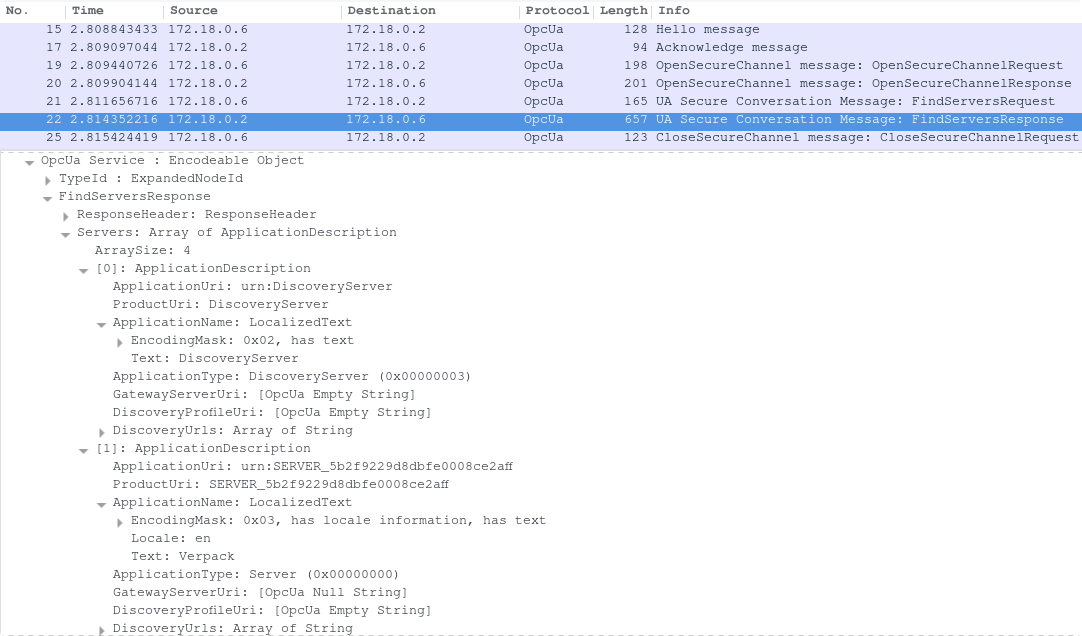
\includegraphics[width=14cm]{opcua-secure-none-res}
  \caption{Paketanalyse OPC UA - Server Response bei Sicherheitsprofil "none"} 
  \label{Analyse:opcua-secure-none-res}
\end{figure}

\begin{figure}[h]
  \centering
  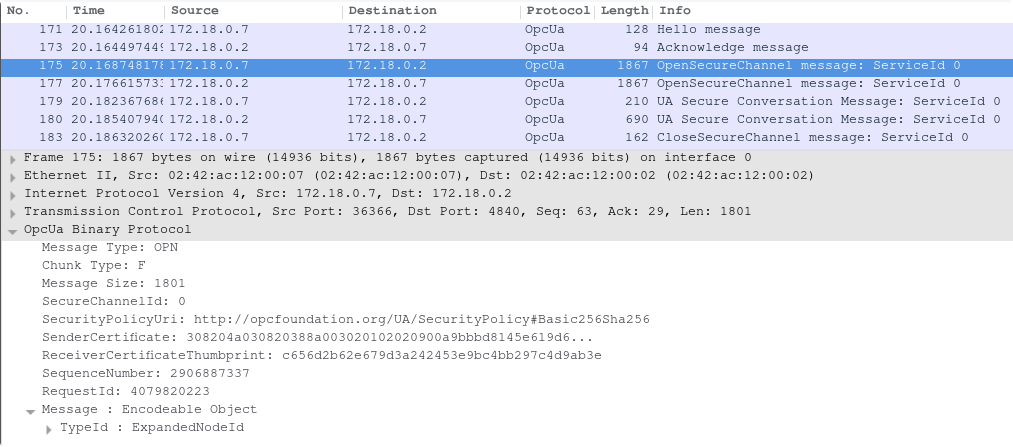
\includegraphics[width=14cm]{opcua-secure-sha-req}
  \caption{Paketanalyse OPC UA - Client Request bei Sicherheitsprofil "Basic256Sha256" und MessageSecurityMode "SIGNANDENCRYPT"} 
  \label{Analyse:opcua-secure-sha-req}
\end{figure}

\begin{figure}[h]
  \centering
  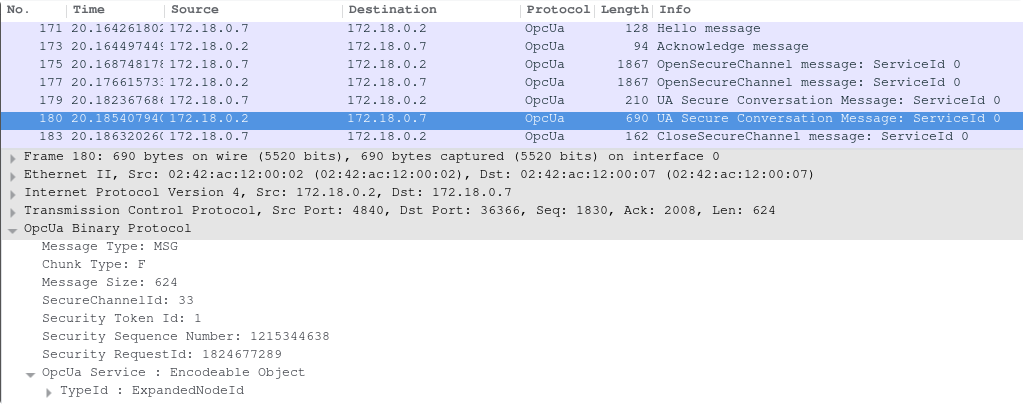
\includegraphics[width=14cm]{opcua-secure-sha-res}
  \caption{Paketanalyse OPC UA - Server Response bei Sicherheitsprofil "Basic256Sha256" und MessageSecurityMode "SIGNANDENCRYPT"} 
  \label{Analyse:opcua-secure-sha-res}
\end{figure}

Das in \autoref{Anwendungsszenarien:MitM} beschriebene Anwendungsszenario des \ac{MitM} Angriffs kann ebenfalls mit Hilfe eine Paketanalyse durchgeführt werden. Hierzu müssen die Pakete der Netzwerkschnittstelle des Netzwerks "`i40-network"' der \ac{VM} "`i40"' abgehört werden. Nach Aktivierung des Rogue \ac{DHCP} Servers, der Aktualisierung der \ac{DHCP} Konfiguration des Netzwerkadapters der \ac{VM} "`comp"' und der gleichzeitigen Änderung des Standardgateways ist es möglich die Netzwerkpakete des in der \ac{VM} simulierten Temperatursensors und dessen Empfängeradresse mitzulesen. \autoref{arg} stellt den Zugriff auf die Netzwerkpakete, welche für ein anderes Netz bestimmt sind, dar.

TODO - Screenshot

Das Anwendungsszenario der Manipulation des Monitoringsystems (\autoref{Anwendungsszenarien:Manipulation von ungesichertem Netzwerkverkehr}) dient der Visualisierung der Auswirkungen eines \ac{MitM} Angriffs und der Darstellung eines Angriffsszenarios durch die gewonnen Daten. Die durch die \ac{MitM} gewonnene Empfängeradresse des \ac{CoAP} Servers wird genutzt, um diesem selbst Pakete unter dem selben Topic zuzusenden und somit die Temperaturdaten des Sensors im Monitoringsystem zu beeinflussen. Dem Monitoringsystem werden hohe Temperaturen des Sensors zugesendet, um dort einen Alarm auszulösen und somit den Produktionsprozess zu manipulieren.

TODO - Screenshot GUI Alarm